\begin{defn}[Walks and their Kin] In graph theory we frequently study movement in a graph, for that we need the following definitions.
\index{walk}\index{trail}\index{circuit}\index{simple circuit}\index{Euler circuit}\index{Euler trail}\index{Hamilton circuit}\index{closed walk}\index{path}
\begin{sides}[lefthand width=0.4\linewidth]
\begin{center}
    % \inputtikz{graph_walk_types}
    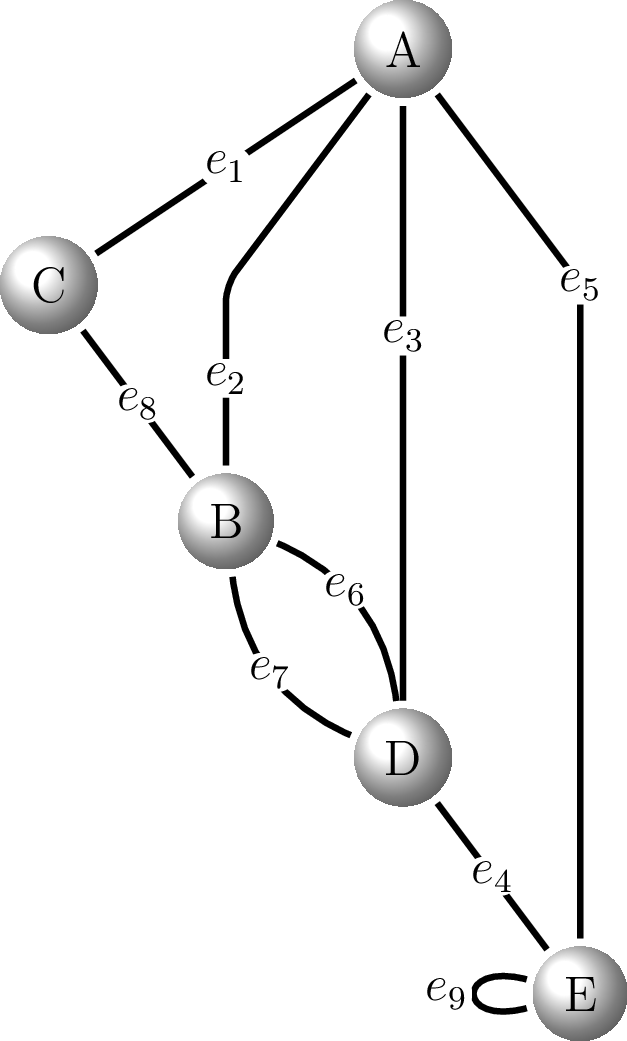
\includegraphics[scale=0.24,alt={graph use to discuss different types of walks}]{images/created/graph_walk_types.png}
\end{center}    

\tcblower

\begin{itemize}
    \item \emph{Walk:} Finite sequence of vertices and edges.\vspace{0.7\baselineskip}\newline\rule{0.8\linewidth}{0.2pt}
    \item \emph{Trail:} A walk with no repeated edges.\vspace{0.7\baselineskip}\newline\rule{0.8\linewidth}{0.2pt}
    \item \emph{Euler Trail:} A trail that traverses every edge.\vspace{0.7\baselineskip}\newline\rule{0.8\linewidth}{0.2pt}
    \item \emph{Circuit:} A non-trivial closed trail.\vspace{0.7\baselineskip}\newline\rule{0.8\linewidth}{0.2pt}
    \item \emph{Euler Circuit:} Circuit that traverses every edge.\vspace{0.7\baselineskip}\newline\rule{0.8\linewidth}{0.2pt}
    \item \emph{Simple Circuit:} Circuit that only repeats the first/last vertex.\vspace{0.7\baselineskip}\newline\rule{0.8\linewidth}{0.2pt}
    \item \emph{Hamilton Circuit:} A simple circuit that includes every vertex.\vspace{0.7\baselineskip}\newline\rule{0.8\linewidth}{0.2pt}
\end{itemize}
\end{sides}
\begin{figure}[H]
    \centering
    % \inputtikz{graph_walk_relations}
    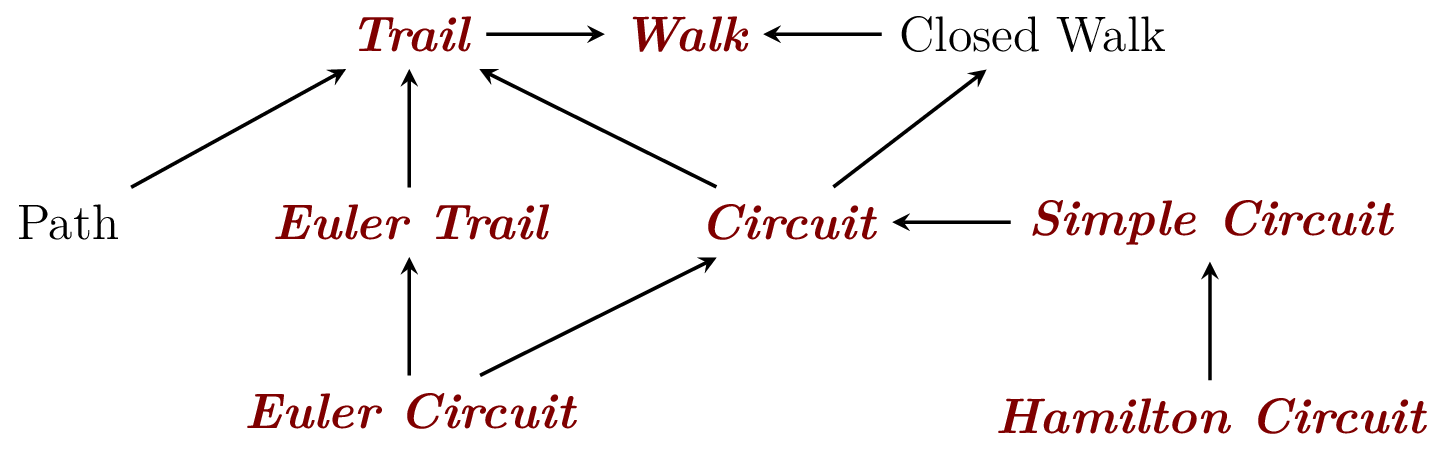
\includegraphics[scale=0.24,alt={graph demonstrating how the different types of walks relate}]{images/created/graph_walk_relations.png}
    % \includegraphics[width=0.5\linewidth]{}
    \caption{Hierarchy of Walks in a Graph}
    \label{fig:walk-types}
\end{figure}
\end{defn}

\clearpage

\begin{practiceprob}\index{Euler circuit}\index{Euler trail}\index{Hamilton circuit}
Try and determine if the graph below has an:
\begin{itemize}
    \item \emph{Euler Trail:} A trail that traverses every edge.\vspace{0.7\baselineskip}\newline\rule{0.8\linewidth}{0.2pt}
    \item \emph{Euler Circuit:} Circuit that traverses every edge.\vspace{0.7\baselineskip}\newline\rule{0.8\linewidth}{0.2pt}
    \item \emph{Hamilton Circuit:} A simple circuit that includes every vertex.\vspace{0.7\baselineskip}\newline\rule{0.8\linewidth}{0.2pt}
\end{itemize}

\begin{center}
    % \inputtikz{graph_euler_pract1}
    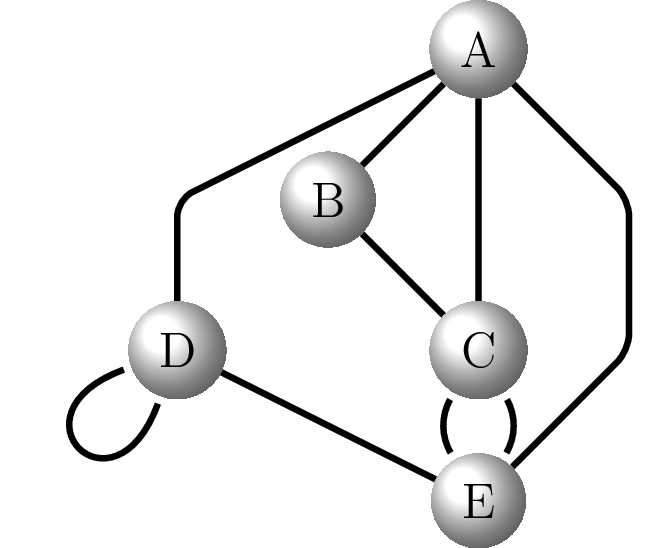
\includegraphics[scale=0.24,alt={practice graph for finind Euler circuits}]{images/created/graph_euler_pract1.png}
\end{center}
\end{practiceprob}

\begin{practiceprob}\index{Euler circuit}\index{Euler trail}\index{Hamilton circuit}
Try and determine if the graph below has an:
\begin{itemize}
    \item \emph{Euler Trail:} A trail that traverses every edge.\vspace{0.7\baselineskip}\newline\rule{0.8\linewidth}{0.2pt}
    \item \emph{Euler Circuit:} Circuit that traverses every edge.\vspace{0.7\baselineskip}\newline\rule{0.8\linewidth}{0.2pt}
    \item \emph{Hamilton Circuit:} A simple circuit that includes every vertex.\vspace{0.7\baselineskip}\newline\rule{0.8\linewidth}{0.2pt}
\end{itemize}

\begin{center}
    % \inputtikz{graph_euler_pract2}
    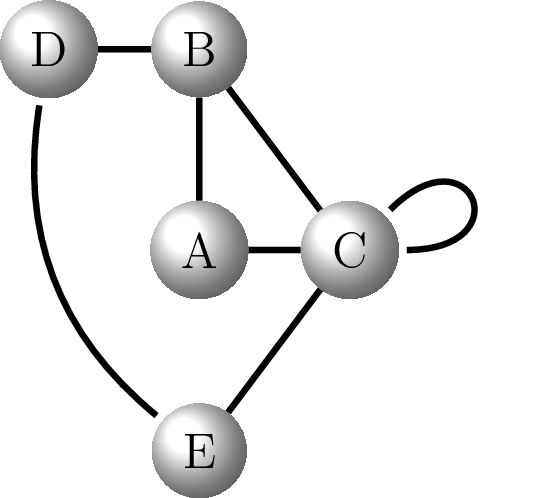
\includegraphics[scale=0.24,alt={practice graph for finind Euler circuits}]{images/created/graph_euler_pract2.png}
\end{center}
\end{practiceprob}



\begin{thm}\index{Euler circuit}\index{Euler trail}\index{Hamilton circuit}
    A connected graph \(G\) will have an \emph{Euler circuit} if all of its vertices are of even degree and only an \emph{Euler trail} if it has exactly two vertices of odd degree.
\end{thm}

\begin{thm}[Subgraphs and Hamilton Circuits]
    If a connected graph \(G\) has a \emph{Hamilton circuit}, then \(G\) has a \emph{subgraph} with the following properties:
    \begin{enumerate}
        \item \(H\) contains every vertex of \(G\).
        \item \(H\) is connected.
        \item \(H\) has an equal number of vertices and edges.
        \item Every vertex in \(H\) has degree 2.
    \end{enumerate}
\end{thm}

\begin{figure}[H]
    \centering
    % \inputtikz{graph_euler_hamilton_thms}
    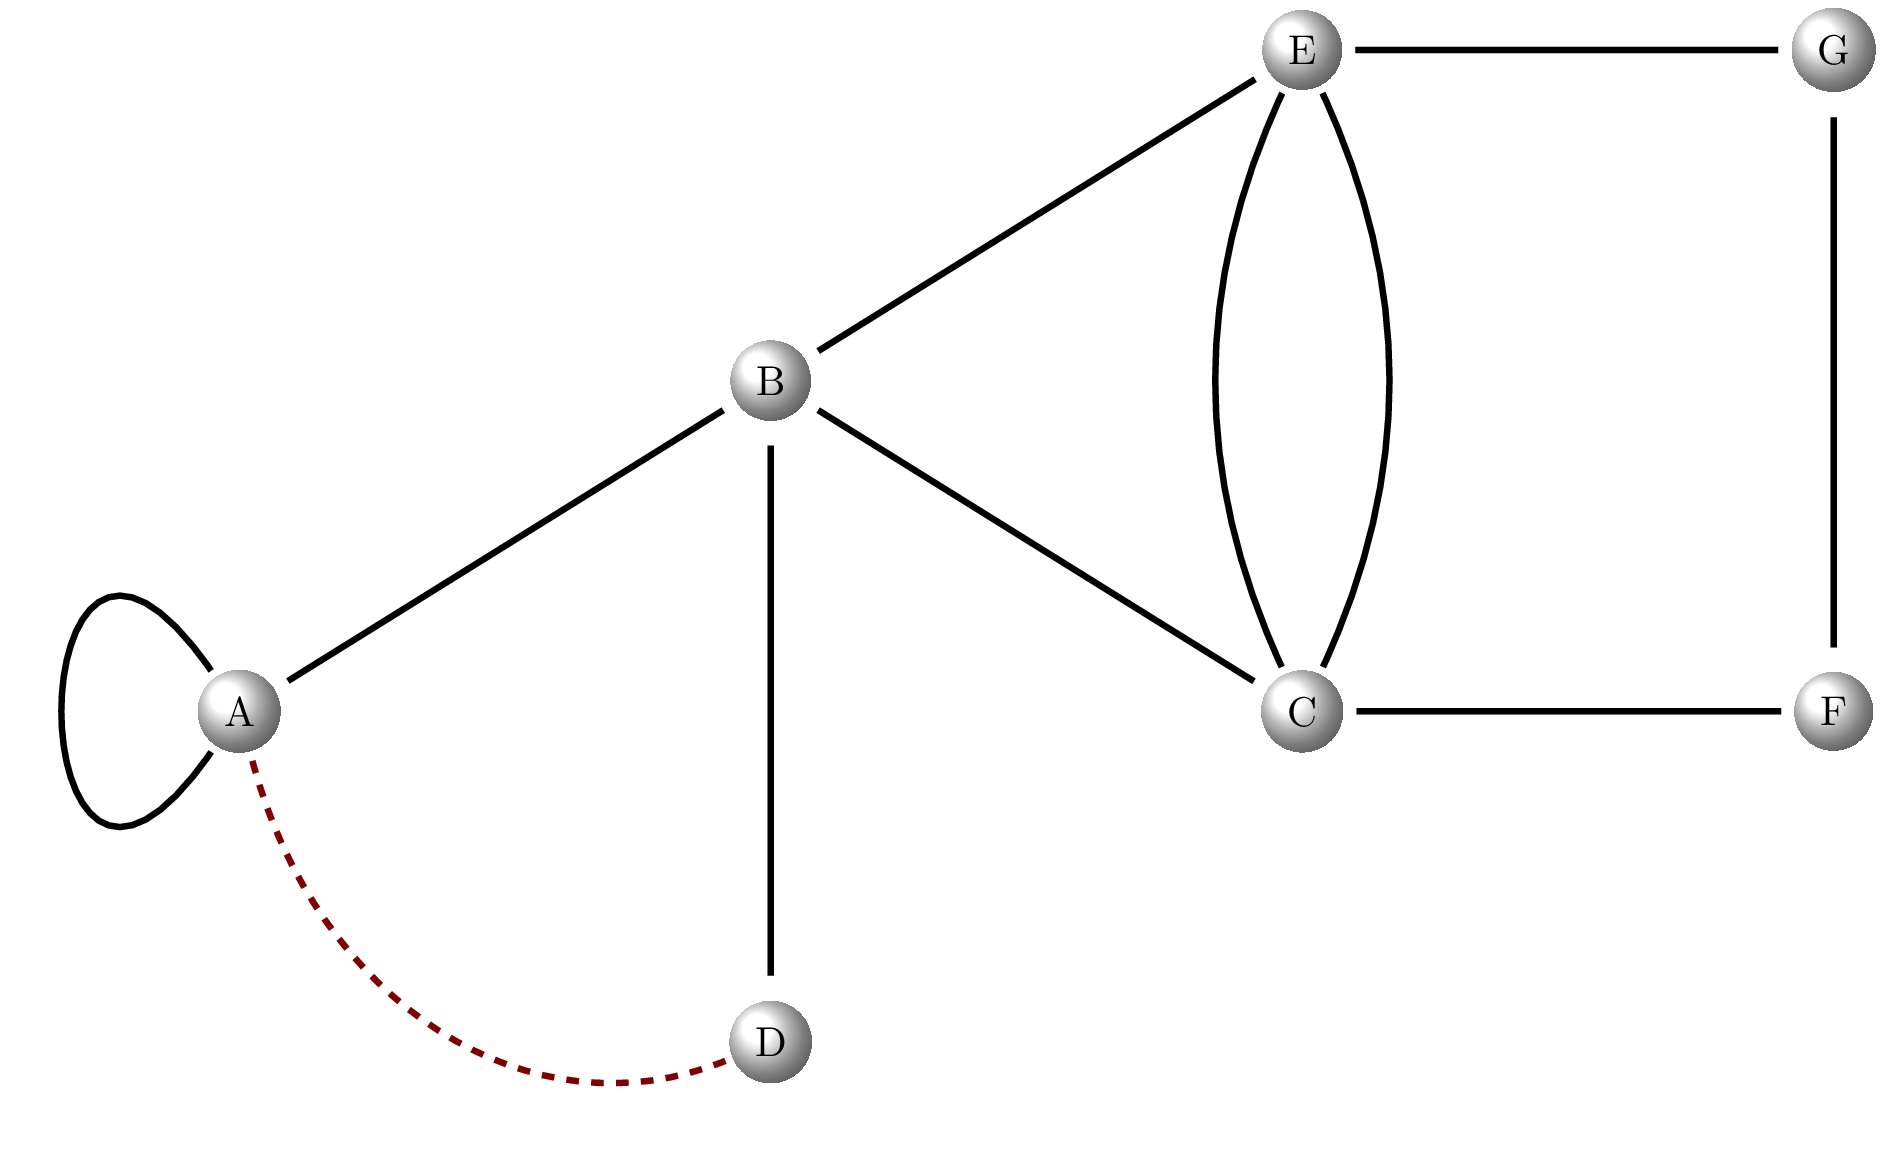
\includegraphics[scale=0.24,alt={practice graph for finind Euler circuits or Hamilton circuits}]{images/created/graph_euler_hamilton_thms.png}
    % \includegraphics[width=0.5\linewidth]{}
    \caption{Euler and Hamilton Circuits}
    \label{fig:euler-hamilton-graph}
\end{figure}

\begin{practiceprob}\index{Euler circuit}\index{Euler trail}\index{Hamilton circuit}
Again try to find any Euler or Hamilton Circuits.

    % \inputtikz{graph_euler_pract3}
    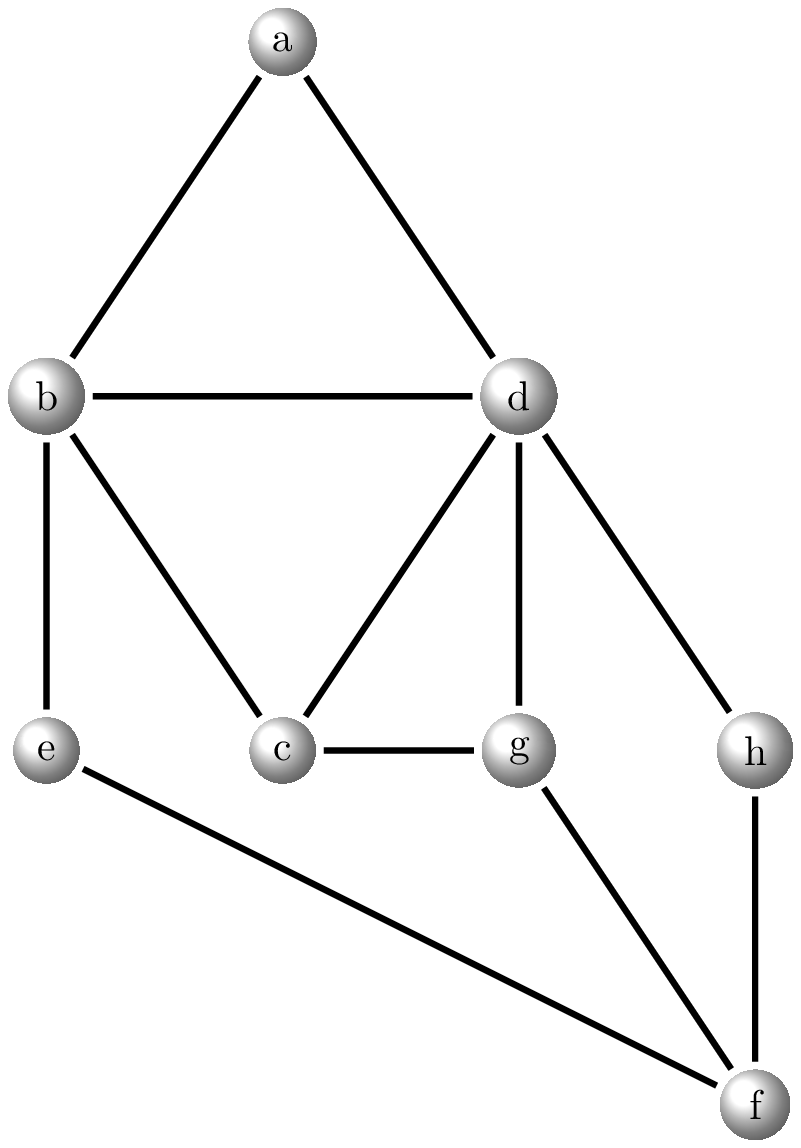
\includegraphics[scale=0.24,alt={practice graph for finind Euler circuits or Hamilton circuits}]{images/created/graph_euler_pract3.png}
\end{practiceprob}

\begin{practiceprob}
Again try to find any Euler or Hamilton Circuits.

    % \inputtikz{graph_euler_pract4}
    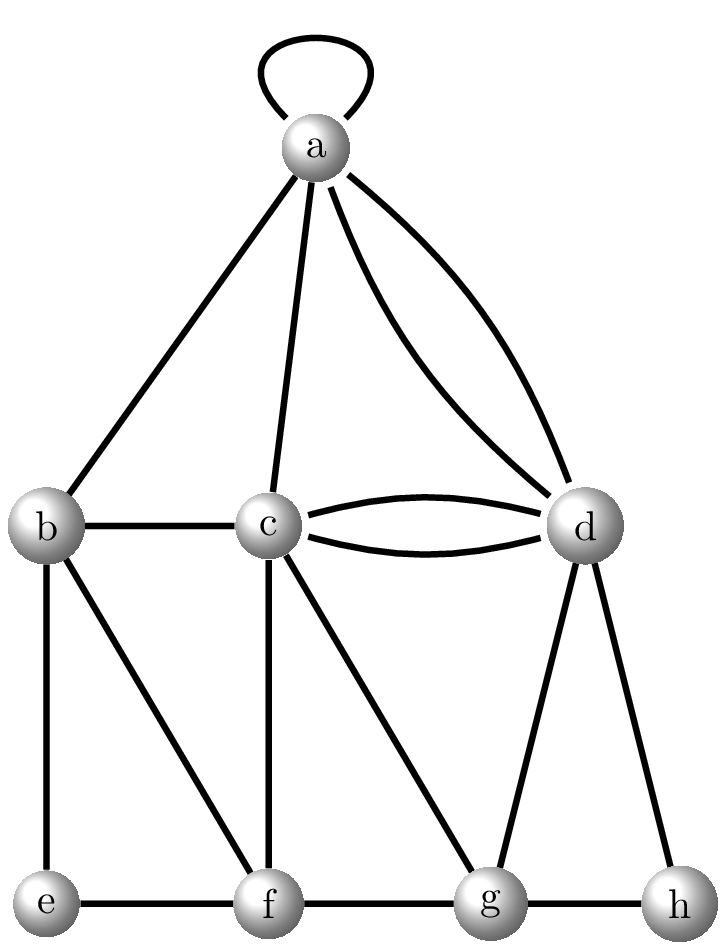
\includegraphics[scale=0.24,alt={practice graph for finind Euler circuits or Hamilton circuits}]{images/created/graph_euler_pract4.png}
\end{practiceprob}





